\documentclass[handout,aspectratio=169]{beamer}
\usepackage[english]{babel}
\usepackage{metalogo}
\usepackage{listings}
\usepackage{fontspec}
\usepackage{tikz}
\usepackage{graphicx}
\usepackage{subcaption}
%%%%%%%%%%%%%%%%%%%%%%%%%%%%%%%%%%%%%%%%%%%%%%%%%%%%%%%%%%%%%%%%%%%%%%%%%%%%%%%%%%%%%%%%
%%%%%%%%%%%%%%%%%%%%%%%%%%%%%%%%%%%%%%%%%%%%%%%%%%%%%%%%%%%%%%%%%%%%%%%%%%%%%%%%%%%%%%%%
%%%%%%%%%%%%%%%%%%%%%%%%%%%%%%%%%%%%%%%%%%%%%%%%%%%%%%%%%%%%%%%%%%%%%%%%%%%%%%%%%%%%%%%%
\usepackage{xcolor}
\definecolor{BK}{HTML}{3b3838}
\definecolor{Blue}{RGB}{88, 105, 225}
\newcommand{\BK}[1]{\color{BK} #1}
\newcommand{\URed}[1]{\color{URed} #1}
\newcommand{\white}[1]{\color{white} #1}
\newcommand{\Orange}[1]{\color{QOrange} #1}
\newcommand{\blue}[1]{\color{blue} #1}
\newcommand{\Blue}[1]{\color{Blue} #1}
\newcommand{\red}[1]{\color{red} #1}
\newcommand{\gray}[1]{\color{gray} #1}
\newcommand{\orange}[1]{\color{orange} #1}
\usepackage{accents}
\newcommand\thickbar[1]{\accentset{\rule{.4em}{.8pt}}{#1}}
\newcommand{\ubar}[1]{\underaccent{\bar}{#1}}
\newcommand{\hatbar}[1]{\bar{\hat{#1}}}
\newcommand{\hatubar}[1]{\underaccent{\bar}{\hat{#1}}}
\newcommand{\ul}[1]{\underline{#1}}
\newcommand{\ol}[1]{\overline{#1}}
%%%%%%%%%%%%%%%%%%%%%%%%%%%%%%%%%%%%%%%%%%%%%%%%%%%%%%%%%%%%%%%%%%%%%%%%%%%%%%%%%%%%%%%%
\newcommand{\bO}[1]{\bf \Orange #1}
%%%%%%%%%%%%%%%%%%%%%%%%%%%%%%%%%%%%%%%%%%%%%%%%%%%%%%%%%%%%%%%%%%%%%%%%%%%%%%%%%%%%%%%%
%%%%%%%%%%%%%%%%%%%%%%%%%%%%%%%%%%%%%%%%%%%%%%%%%%%%%%%%%%%%%%%%%%%%%%%%%%%%%%%%%%%%%%%%
\newcommand{\YBox}[3]{
\begin{center}
\begin{minipage}{#1\linewidth}
\begin{exampleblock}{#2}
    #3
\end{exampleblock}
\end{minipage}
\end{center}
}

\newcommand{\OBox}[3]{
\begin{center}
\begin{minipage}{#1\linewidth}
\begin{block}{#2}
    #3
\end{block}
\end{minipage}
\end{center}
}

\newcommand{\Columns}[4]{
\begin{columns}
\begin{column}{#1\textwidth}
#2
\end{column}
\begin{column}{#3\textwidth}  %%<--- here
#4
\end{column}
\end{columns}
}
%%%%% NEW MATH DEFINITIONS %%%%%

\usepackage{amsmath,amsfonts,bm}
\usepackage{amssymb}

%%%%%%%%%%%%%%%%%%%%%%%%%%%%%%%%%%%%%%%%%%%%%%%%%%%%%%%%%%%%%%%%%%%%%%%%%%%%%%%%
%%%%%%%%%%%%%%%%%%%%%%%%%%%%%%%%%%%%%%%%%%%%%%%%%%%%%%%%%%%%%%%%%%%%%%%%%%%%%%%%
\usepackage{natbib}
\usepackage{ulem}
% \usepackage{cite}
\usepackage{amsmath,amssymb,amsfonts}
\usepackage{algorithm,algorithmicx,algpseudocode}
\usepackage{graphicx}
% \usepackage{subcaption}
\usepackage{mwe}
\usepackage{textcomp}
\usepackage{xcolor}
\usepackage{dsfont}
\usepackage{bbm}
% Mark sections of captions for referring to divisions of figures
\newcommand{\figleft}{{\em (Left)}}
\newcommand{\figcenter}{{\em (Center)}}
\newcommand{\figright}{{\em (Right)}}
\newcommand{\figtop}{{\em (Top)}}
\newcommand{\figbottom}{{\em (Bottom)}}
\newcommand{\captiona}{{\em (a)}}
\newcommand{\captionb}{{\em (b)}}
\newcommand{\captionc}{{\em (c)}}
\newcommand{\captiond}{{\em (d)}}

% Highlight a newly defined term
\newcommand{\newterm}[1]{{\bf #1}}


% Figure reference, lower-case.
\def\figref#1{figure~\ref{#1}}
% Figure reference, capital. For start of sentence
\def\Figref#1{Figure~\ref{#1}}
\def\twofigref#1#2{figures \ref{#1} and \ref{#2}}
\def\quadfigref#1#2#3#4{figures \ref{#1}, \ref{#2}, \ref{#3} and \ref{#4}}
% Section reference, lower-case.
\def\secref#1{section~\ref{#1}}
% Section reference, capital.
\def\Secref#1{Section~\ref{#1}}
% Reference to two sections.
\def\twosecrefs#1#2{sections \ref{#1} and \ref{#2}}
% Reference to three sections.
\def\secrefs#1#2#3{sections \ref{#1}, \ref{#2} and \ref{#3}}
% Reference to an equation, lower-case.
\def\eqref#1{equation~\ref{#1}}
% Reference to an equation, upper case
\def\Eqref#1{Equation~\ref{#1}}
% A raw reference to an equation---avoid using if possible
\def\plaineqref#1{\ref{#1}}
% Reference to a chapter, lower-case.
\def\chapref#1{chapter~\ref{#1}}
% Reference to an equation, upper case.
\def\Chapref#1{Chapter~\ref{#1}}
% Reference to a range of chapters
\def\rangechapref#1#2{chapters\ref{#1}--\ref{#2}}
% Reference to an algorithm, lower-case.
\def\algref#1{algorithm~\ref{#1}}
% Reference to an algorithm, upper case.
\def\Algref#1{Algorithm~\ref{#1}}
\def\twoalgref#1#2{algorithms \ref{#1} and \ref{#2}}
\def\Twoalgref#1#2{Algorithms \ref{#1} and \ref{#2}}
% Reference to a part, lower case
\def\partref#1{part~\ref{#1}}
% Reference to a part, upper case
\def\Partref#1{Part~\ref{#1}}
\def\twopartref#1#2{parts \ref{#1} and \ref{#2}}

\def\ceil#1{\lceil #1 \rceil}
\def\floor#1{\lfloor #1 \rfloor}
\def\1{\bm{1}}
\newcommand{\train}{\mathcal{D}}
\newcommand{\valid}{\mathcal{D_{\mathrm{valid}}}}
\newcommand{\test}{\mathcal{D_{\mathrm{test}}}}

\def\eps{{\epsilon}}


% Random variables
\def\reta{{\textnormal{$\eta$}}}
\def\ra{{\textnormal{a}}}
\def\rb{{\textnormal{b}}}
\def\rc{{\textnormal{c}}}
\def\rd{{\textnormal{d}}}
\def\re{{\textnormal{e}}}
\def\rf{{\textnormal{f}}}
\def\rg{{\textnormal{g}}}
\def\rh{{\textnormal{h}}}
\def\ri{{\textnormal{i}}}
\def\rj{{\textnormal{j}}}
\def\rk{{\textnormal{k}}}
\def\rl{{\textnormal{l}}}
% rm is already a command, just don't name any random variables m
\def\rn{{\textnormal{n}}}
\def\ro{{\textnormal{o}}}
\def\rp{{\textnormal{p}}}
\def\rq{{\textnormal{q}}}
\def\rr{{\textnormal{r}}}
\def\rs{{\textnormal{s}}}
\def\rt{{\textnormal{t}}}
\def\ru{{\textnormal{u}}}
\def\rv{{\textnormal{v}}}
\def\rw{{\textnormal{w}}}
\def\rx{{\textnormal{x}}}
\def\ry{{\textnormal{y}}}
\def\rz{{\textnormal{z}}}

% Random vectors
\def\rvepsilon{{\mathbf{\epsilon}}}
\def\rvtheta{{\mathbf{\theta}}}
\def\rva{{\mathbf{a}}}
\def\rvb{{\mathbf{b}}}
\def\rvc{{\mathbf{c}}}
\def\rvd{{\mathbf{d}}}
\def\rve{{\mathbf{e}}}
\def\rvf{{\mathbf{f}}}
\def\rvg{{\mathbf{g}}}
\def\rvh{{\mathbf{h}}}
\def\rvu{{\mathbf{i}}}
\def\rvj{{\mathbf{j}}}
\def\rvk{{\mathbf{k}}}
\def\rvl{{\mathbf{l}}}
\def\rvm{{\mathbf{m}}}
\def\rvn{{\mathbf{n}}}
\def\rvo{{\mathbf{o}}}
\def\rvp{{\mathbf{p}}}
\def\rvq{{\mathbf{q}}}
\def\rvr{{\mathbf{r}}}
\def\rvs{{\mathbf{s}}}
\def\rvt{{\mathbf{t}}}
\def\rvu{{\mathbf{u}}}
\def\rvv{{\mathbf{v}}}
\def\rvw{{\mathbf{w}}}
\def\rvx{{\mathbf{x}}}
\def\rvy{{\mathbf{y}}}
\def\rvz{{\mathbf{z}}}

% Elements of random vectors
\def\erva{{\textnormal{a}}}
\def\ervb{{\textnormal{b}}}
\def\ervc{{\textnormal{c}}}
\def\ervd{{\textnormal{d}}}
\def\erve{{\textnormal{e}}}
\def\ervf{{\textnormal{f}}}
\def\ervg{{\textnormal{g}}}
\def\ervh{{\textnormal{h}}}
\def\ervi{{\textnormal{i}}}
\def\ervj{{\textnormal{j}}}
\def\ervk{{\textnormal{k}}}
\def\ervl{{\textnormal{l}}}
\def\ervm{{\textnormal{m}}}
\def\ervn{{\textnormal{n}}}
\def\ervo{{\textnormal{o}}}
\def\ervp{{\textnormal{p}}}
\def\ervq{{\textnormal{q}}}
\def\ervr{{\textnormal{r}}}
\def\ervs{{\textnormal{s}}}
\def\ervt{{\textnormal{t}}}
\def\ervu{{\textnormal{u}}}
\def\ervv{{\textnormal{v}}}
\def\ervw{{\textnormal{w}}}
\def\ervx{{\textnormal{x}}}
\def\ervy{{\textnormal{y}}}
\def\ervz{{\textnormal{z}}}

% Random matrices
\def\rmA{{\mathbf{A}}}
\def\rmB{{\mathbf{B}}}
\def\rmC{{\mathbf{C}}}
\def\rmD{{\mathbf{D}}}
\def\rmE{{\mathbf{E}}}
\def\rmF{{\mathbf{F}}}
\def\rmG{{\mathbf{G}}}
\def\rmH{{\mathbf{H}}}
\def\rmI{{\mathbf{I}}}
\def\rmJ{{\mathbf{J}}}
\def\rmK{{\mathbf{K}}}
\def\rmL{{\mathbf{L}}}
\def\rmM{{\mathbf{M}}}
\def\rmN{{\mathbf{N}}}
\def\rmO{{\mathbf{O}}}
\def\rmP{{\mathbf{P}}}
\def\rmQ{{\mathbf{Q}}}
\def\rmR{{\mathbf{R}}}
\def\rmS{{\mathbf{S}}}
\def\rmT{{\mathbf{T}}}
\def\rmU{{\mathbf{U}}}
\def\rmV{{\mathbf{V}}}
\def\rmW{{\mathbf{W}}}
\def\rmX{{\mathbf{X}}}
\def\rmY{{\mathbf{Y}}}
\def\rmZ{{\mathbf{Z}}}

% Elements of random matrices
\def\ermA{{\textnormal{A}}}
\def\ermB{{\textnormal{B}}}
\def\ermC{{\textnormal{C}}}
\def\ermD{{\textnormal{D}}}
\def\ermE{{\textnormal{E}}}
\def\ermF{{\textnormal{F}}}
\def\ermG{{\textnormal{G}}}
\def\ermH{{\textnormal{H}}}
\def\ermI{{\textnormal{I}}}
\def\ermJ{{\textnormal{J}}}
\def\ermK{{\textnormal{K}}}
\def\ermL{{\textnormal{L}}}
\def\ermM{{\textnormal{M}}}
\def\ermN{{\textnormal{N}}}
\def\ermO{{\textnormal{O}}}
\def\ermP{{\textnormal{P}}}
\def\ermQ{{\textnormal{Q}}}
\def\ermR{{\textnormal{R}}}
\def\ermS{{\textnormal{S}}}
\def\ermT{{\textnormal{T}}}
\def\ermU{{\textnormal{U}}}
\def\ermV{{\textnormal{V}}}
\def\ermW{{\textnormal{W}}}
\def\ermX{{\textnormal{X}}}
\def\ermY{{\textnormal{Y}}}
\def\ermZ{{\textnormal{Z}}}

% Vectors
\def\vzero{{\bm{0}}}
\def\vone{{\bm{1}}}
\def\vmu{{\bm{\mu}}}
\def\vtheta{{\bm{\theta}}}
\def\va{{\bm{a}}}
\def\vb{{\bm{b}}}
\def\vc{{\bm{c}}}
\def\vd{{\bm{d}}}
\def\ve{{\bm{e}}}
\def\vf{{\bm{f}}}
\def\vg{{\bm{g}}}
\def\vh{{\bm{h}}}
\def\vi{{\bm{i}}}
\def\vj{{\bm{j}}}
\def\vk{{\bm{k}}}
\def\vl{{\bm{l}}}
\def\vm{{\bm{m}}}
\def\vn{{\bm{n}}}
\def\vo{{\bm{o}}}
\def\vp{{\bm{p}}}
\def\vq{{\bm{q}}}
\def\vr{{\bm{r}}}
\def\vs{{\bm{s}}}
\def\vt{{\bm{t}}}
\def\vu{{\bm{u}}}
\def\vv{{\bm{v}}}
\def\vw{{\bm{w}}}
\def\vx{{\bm{x}}}
\def\vy{{\bm{y}}}
\def\vz{{\bm{z}}}

% Elements of vectors
\def\evalpha{{\alpha}}
\def\evbeta{{\beta}}
\def\evepsilon{{\epsilon}}
\def\evlambda{{\lambda}}
\def\evomega{{\omega}}
\def\evmu{{\mu}}
\def\evpsi{{\psi}}
\def\evsigma{{\sigma}}
\def\evtheta{{\theta}}
\def\eva{{a}}
\def\evb{{b}}
\def\evc{{c}}
\def\evd{{d}}
\def\eve{{e}}
\def\evf{{f}}
\def\evg{{g}}
\def\evh{{h}}
\def\evi{{i}}
\def\evj{{j}}
\def\evk{{k}}
\def\evl{{l}}
\def\evm{{m}}
\def\evn{{n}}
\def\evo{{o}}
\def\evp{{p}}
\def\evq{{q}}
\def\evr{{r}}
\def\evs{{s}}
\def\evt{{t}}
\def\evu{{u}}
\def\evv{{v}}
\def\evw{{w}}
\def\evx{{x}}
\def\evy{{y}}
\def\evz{{z}}

% Matrix
\def\mA{{\bm{A}}}
\def\mB{{\bm{B}}}
\def\mC{{\bm{C}}}
\def\mD{{\bm{D}}}
\def\mE{{\bm{E}}}
\def\mF{{\bm{F}}}
\def\mG{{\bm{G}}}
\def\mH{{\bm{H}}}
\def\mI{{\bm{I}}}
\def\mJ{{\bm{J}}}
\def\mK{{\bm{K}}}
\def\mL{{\bm{L}}}
\def\mM{{\bm{M}}}
\def\mN{{\bm{N}}}
\def\mO{{\bm{O}}}
\def\mP{{\bm{P}}}
\def\mQ{{\bm{Q}}}
\def\mR{{\bm{R}}}
\def\mS{{\bm{S}}}
\def\mT{{\bm{T}}}
\def\mU{{\bm{U}}}
\def\mV{{\bm{V}}}
\def\mW{{\bm{W}}}
\def\mX{{\bm{X}}}
\def\mY{{\bm{Y}}}
\def\mZ{{\bm{Z}}}
\def\mBeta{{\bm{\beta}}}
\def\mPhi{{\bm{\Phi}}}
\def\mLambda{{\bm{\Lambda}}}
\def\mSigma{{\bm{\Sigma}}}

% Tensor
\DeclareMathAlphabet{\mathsfit}{\encodingdefault}{\sfdefault}{m}{sl}
\SetMathAlphabet{\mathsfit}{bold}{\encodingdefault}{\sfdefault}{bx}{n}
\newcommand{\tens}[1]{\bm{\mathsfit{#1}}}
\def\tA{{\tens{A}}}
\def\tB{{\tens{B}}}
\def\tC{{\tens{C}}}
\def\tD{{\tens{D}}}
\def\tE{{\tens{E}}}
\def\tF{{\tens{F}}}
\def\tG{{\tens{G}}}
\def\tH{{\tens{H}}}
\def\tI{{\tens{I}}}
\def\tJ{{\tens{J}}}
\def\tK{{\tens{K}}}
\def\tL{{\tens{L}}}
\def\tM{{\tens{M}}}
\def\tN{{\tens{N}}}
\def\tO{{\tens{O}}}
\def\tP{{\tens{P}}}
\def\tQ{{\tens{Q}}}
\def\tR{{\tens{R}}}
\def\tS{{\tens{S}}}
\def\tT{{\tens{T}}}
\def\tU{{\tens{U}}}
\def\tV{{\tens{V}}}
\def\tW{{\tens{W}}}
\def\tX{{\tens{X}}}
\def\tY{{\tens{Y}}}
\def\tZ{{\tens{Z}}}


% Graph
\def\gA{{\mathcal{A}}}
\def\gB{{\mathcal{B}}}
\def\gC{{\mathcal{C}}}
\def\gD{{\mathcal{D}}}
\def\gE{{\mathcal{E}}}
\def\gF{{\mathcal{F}}}
\def\gG{{\mathcal{G}}}
\def\gH{{\mathcal{H}}}
\def\gI{{\mathcal{I}}}
\def\gJ{{\mathcal{J}}}
\def\gK{{\mathcal{K}}}
\def\gL{{\mathcal{L}}}
\def\gM{{\mathcal{M}}}
\def\gN{{\mathcal{N}}}
\def\gO{{\mathcal{O}}}
\def\gP{{\mathcal{P}}}
\def\gQ{{\mathcal{Q}}}
\def\gR{{\mathcal{R}}}
\def\gS{{\mathcal{S}}}
\def\gT{{\mathcal{T}}}
\def\gU{{\mathcal{U}}}
\def\gV{{\mathcal{V}}}
\def\gW{{\mathcal{W}}}
\def\gX{{\mathcal{X}}}
\def\gY{{\mathcal{Y}}}
\def\gZ{{\mathcal{Z}}}

% Sets
\def\sA{{\mathbb{A}}}
\def\sB{{\mathbb{B}}}
\def\sC{{\mathbb{C}}}
\def\sD{{\mathbb{D}}}
% Don't use a set called E, because this would be the same as our symbol
% for expectation.
\def\sF{{\mathbb{F}}}
\def\sG{{\mathbb{G}}}
\def\sH{{\mathbb{H}}}
\def\sI{{\mathbb{I}}}
\def\sJ{{\mathbb{J}}}
\def\sK{{\mathbb{K}}}
\def\sL{{\mathbb{L}}}
\def\sM{{\mathbb{M}}}
\def\sN{{\mathbb{N}}}
\def\sO{{\mathbb{O}}}
\def\sP{{\mathbb{P}}}
\def\sQ{{\mathbb{Q}}}
\def\sR{{\mathbb{R}}}
\def\sS{{\mathbb{S}}}
\def\sT{{\mathbb{T}}}
\def\sU{{\mathbb{U}}}
\def\sV{{\mathbb{V}}}
\def\sW{{\mathbb{W}}}
\def\sX{{\mathbb{X}}}
\def\sY{{\mathbb{Y}}}
\def\sZ{{\mathbb{Z}}}

% Entries of a matrix
\def\emLambda{{\Lambda}}
\def\emA{{A}}
\def\emB{{B}}
\def\emC{{C}}
\def\emD{{D}}
\def\emE{{E}}
\def\emF{{F}}
\def\emG{{G}}
\def\emH{{H}}
\def\emI{{I}}
\def\emJ{{J}}
\def\emK{{K}}
\def\emL{{L}}
\def\emM{{M}}
\def\emN{{N}}
\def\emO{{O}}
\def\emP{{P}}
\def\emQ{{Q}}
\def\emR{{R}}
\def\emS{{S}}
\def\emT{{T}}
\def\emU{{U}}
\def\emV{{V}}
\def\emW{{W}}
\def\emX{{X}}
\def\emY{{Y}}
\def\emZ{{Z}}
\def\emSigma{{\Sigma}}

% entries of a tensor
% Same font as tensor, without \bm wrapper
\newcommand{\etens}[1]{\mathsfit{#1}}
\def\etLambda{{\etens{\Lambda}}}
\def\etA{{\etens{A}}}
\def\etB{{\etens{B}}}
\def\etC{{\etens{C}}}
\def\etD{{\etens{D}}}
\def\etE{{\etens{E}}}
\def\etF{{\etens{F}}}
\def\etG{{\etens{G}}}
\def\etH{{\etens{H}}}
\def\etI{{\etens{I}}}
\def\etJ{{\etens{J}}}
\def\etK{{\etens{K}}}
\def\etL{{\etens{L}}}
\def\etM{{\etens{M}}}
\def\etN{{\etens{N}}}
\def\etO{{\etens{O}}}
\def\etP{{\etens{P}}}
\def\etQ{{\etens{Q}}}
\def\etR{{\etens{R}}}
\def\etS{{\etens{S}}}
\def\etT{{\etens{T}}}
\def\etU{{\etens{U}}}
\def\etV{{\etens{V}}}
\def\etW{{\etens{W}}}
\def\etX{{\etens{X}}}
\def\etY{{\etens{Y}}}
\def\etZ{{\etens{Z}}}

% The true underlying data generating distribution
\newcommand{\pdata}{p_{\rm{data}}}
% The empirical distribution defined by the training set
\newcommand{\ptrain}{\hat{p}_{\rm{data}}}
\newcommand{\Ptrain}{\hat{P}_{\rm{data}}}
% The model distribution
\newcommand{\pmodel}{p_{\rm{model}}}
\newcommand{\Pmodel}{P_{\rm{model}}}
\newcommand{\ptildemodel}{\tilde{p}_{\rm{model}}}
% Stochastic autoencoder distributions
\newcommand{\pencode}{p_{\rm{encoder}}}
\newcommand{\pdecode}{p_{\rm{decoder}}}
\newcommand{\precons}{p_{\rm{reconstruct}}}

\newcommand{\laplace}{\mathrm{Laplace}} % Laplace distribution

\newcommand{\E}{\mathbb{E}}
\newcommand{\Ls}{\mathcal{L}}
\newcommand{\R}{\mathbb{R}}
\newcommand{\emp}{\tilde{p}}
\newcommand{\lr}{\alpha}
\newcommand{\reg}{\lambda}
\newcommand{\rect}{\mathrm{rectifier}}
\newcommand{\softmax}{\mathrm{softmax}}
\newcommand{\sigmoid}{\sigma}
\newcommand{\softplus}{\zeta}
\newcommand{\KL}{D_{\mathrm{KL}}}
\newcommand{\Var}{\mathrm{Var}}
\newcommand{\standarderror}{\mathrm{SE}}
\newcommand{\Cov}{\mathrm{Cov}}
% Wolfram Mathworld says $L^2$ is for function spaces and $\ell^2$ is for vectors
% But then they seem to use $L^2$ for vectors throughout the site, and so does
% wikipedia.
\newcommand{\normlzero}{L^0}
\newcommand{\normlone}{L^1}
\newcommand{\normltwo}{L^2}
\newcommand{\normlp}{L^p}
\newcommand{\normmax}{L^\infty}

\newcommand{\parents}{Pa} % See usage in notation.tex. Chosen to match Daphne's book.

% \DeclareMathOperator*{\argmax}{arg\,max}
% \DeclareMathOperator*{\argmin}{arg\,min}
\DeclareMathOperator{\arginf}{arg\,inf}
\DeclareMathOperator{\argmin}{arg\,min}
\DeclareMathOperator{\argmax}{arg\,max}
\DeclareMathOperator{\argsup}{arg\,sup}
\DeclareMathOperator*{\diag}{\textit{diag}}
\DeclareMathOperator*{\trace}{\textit{tr}}
\DeclareMathOperator*{\rank}{\textit{rk}}

\DeclareMathOperator{\sign}{sign}
\DeclareMathOperator{\Tr}{Tr}
\let\ab\allowbreak

\usetheme{Nord}
%%%%% \setmainfont{}
\setmainfont{Montserrat}
\setsansfont{Andika New Basic}
\setmonofont{DejaVu Sans Mono}

%%%%%%%%%%%%%%%%%%%%%%%%%%%%%%%%%%%%%%%%%%%%%%%%%%%%%%%%%%%%%%%%%%%%%%%%%%%%%%%%%%%%%%%%
%%%%%%%%%%%%%%%%%%%%%%%%%%%%%%%%%%%%%%%%%%%%%%%%%%%%%%%%%%%%%%%%%%%%%%%%%%%%%%%%%%%%%%%%
\newcommand{\bs}{

\bigskip

}
\newcommand{\ms}{

\medskip

}
%%%%%%%%%%%%%%%%%%%%%%%%%%%%%
\usepackage{tcolorbox}
\newtcolorbox{mybox}{width=9cm, left=0mm,right = 0mm,top=1mm,bottom=1mm,boxsep=0mm}
\newtcolorbox{myboxL}{width=15cm, left=0mm,right = 0mm,top=1mm,bottom=1mm,boxsep=0mm}
\newtcolorbox{mybox1}{width=5.5cm, left=0mm,right = 0mm,top=1mm,bottom=1mm,boxsep=0mm,colback=BK, coltext=QOrange}

\newtcolorbox{mybox2}{width=12cm, left=0mm,right = 0mm,top=1mm,bottom=1mm,boxsep=0mm,colback=BK, coltext=QOrange}

\newtcolorbox{mybox3}{width=3cm, left=0mm,right = 0mm,top=1mm,bottom=1mm,boxsep=0mm,colback=BK, coltext=QOrange}

\newtcolorbox{mybox4}{width=11cm, left=1mm,right = 1mm,top=1mm,bottom=1mm,boxsep=0mm,colback=BK, coltext=QOrange}
%%%%%%%%%%%%%%%%%%%%%%%%%%%%%%%%%%%%%%%%%%%%%%%%%%%%%%%%%%%%%%%%%%%%%%%%%%%%%%%%%%%%%%%%
%%%%%%%%%%%%%%%%%%%%%%%%%%%%%%%%%%%%%%%%%%%%%%%%%%%%%%%%%%%%%%%%%%%%%%%%%%%%%%%%%%%%%%%%

\usepackage{amsmath}
\graphicspath{{figs/fig00/}}
%-----------------
%	TITLE
%-----------------
\title{
Chapter 04: Gaussian Processes \\ Pages: 67-77
}
\author{\bf Notes by Kumar Anurag}
\date{}

%-----------------
%	SUBTITLE
%-----------------
\subtitle{
Probabilistic Artificial Intelligence
}

\begin{document}

%-----------------
%	TITLE PAGE
%-----------------
{\usebackgroundtemplate{
\includegraphics[width=\paperwidth]{chapter_figs/01_figs/titlepic.png}}
	\begin{frame}[plain,noframenumbering]
		\maketitle
	\end{frame}}


%-----------------------
%	PRESENTATION SLIDES
%-----------------------

\begin{frame}{4.4 Model Selection}
\begin{itemize}
    \item So far, we assumed hyperparameters $\boldsymbol{\theta}$ (e.g., kernel parameters) are known.
    \item In practice, we must learn $\boldsymbol{\theta}$ from data.
    \item A common supervised learning technique:
    \begin{itemize}
        \item Pick $\boldsymbol{\theta}$ such that the resulting predictor $\hat{f}_\theta$ performs best on a hold-out validation set.
    \end{itemize}
    \item This is known as \textbf{point estimate-based model selection}.
    \item Later, we’ll contrast it with a fully \textbf{Bayesian approach} that uses the posterior over $f$ instead of a point estimate.
\end{itemize}
\pause
\vspace{0.3cm}

\end{frame}

\begin{frame}{4.4.1 Optimizing Validation Performance}
\begin{itemize}
    \item Split data $\mathcal{D}$ into:
    \begin{itemize}
        \item Training set $\mathcal{D}^{\text{train}} = \{(x^{\text{train}}_i, y^{\text{train}}_i)\}_{i=1}^n$
        \item Validation set $\mathcal{D}^{\text{val}} = \{(x^{\text{val}}_j, y^{\text{val}}_j)\}_{j=1}^m$
    \end{itemize}
    \item Step 1: Train a model $\hat{f}_j$ for some candidate $\theta_j$ on the training set:
    \[
    \hat{f}_j \triangleq \arg\max_f p(f \mid x_{1:n}^{\text{train}}, y_{1:n}^{\text{train}}) \tag{4.22}
    \]
    \item Step 2: Select $\hat{\theta}$ based on validation performance:
    \[
    \hat{\theta} \triangleq \arg\max_{\theta_j} p(y_{1:m}^{\text{val}} \mid x_{1:m}^{\text{val}}, \hat{f}_j) \tag{4.23}
    \]
\end{itemize}
\pause

\end{frame}

\begin{frame}{Why Validation Sets Help: Remark 4.8}
\begin{block}{Approximating Population Risk}
Minimizing loss on the same data used for training often leads to overfitting.

Instead, use independent validation data to estimate risk:
\[
\frac{1}{m} \sum_{i=1}^{m} \ell(y_i^{\text{val}} \mid x_i^{\text{val}}, \hat{f}_j) \approx \mathbb{E}_{(x, y) \sim \mathcal{P}} \left[\ell(y \mid x, \hat{f}_j)\right] \tag{4.24}
\]

\begin{itemize}
    \item This is an empirical approximation of the true population risk.
    \item Helps prevent overfitting and ensures generalization.
\end{itemize}
\end{block}

\pause
\vspace{0.3cm}
\textbf{Limitation:} Still relies on a \textit{point estimate} $\hat{f}_j$. Can we do better?
\end{frame}

\begin{frame}{Maximizing the Marginal Likelihood}
\vspace{-0.2cm}
\begin{itemize}
    \item In Bayesian regression, we don’t want to pick a single function $\hat{f}$.
    \item Instead, we want to score how likely the observed data is under all possible functions defined by kernel parameters $\theta$.
\end{itemize}

\vspace{0.3cm}
\textbf{Marginal likelihood:}
\[
p(y_{1:n} \mid x_{1:n}, \theta) = \int p(y_{1:n} \mid x_{1:n}, f, \theta) \cdot p(f \mid \theta) \, df \tag{4.26}
\]

\pause
\vspace{0.2cm}
\textbf{Key idea:} We integrate over all functions $f$ rather than picking just one.

\vspace{0.3cm}
This gives us a more robust measure of how “compatible” $\theta$ is with the observed data.
\end{frame}


\begin{frame}{Why This Works — Intuition Behind the Math}
\textbf{Marginal likelihood prefers models that:}
\begin{itemize}
    \item Fit the data well \rightarrow  \, high likelihood
    \item Are not overly complex \rightarrow \, high prior probability
\end{itemize}

\begin{columns}
    \column{0.6\textwidth}
    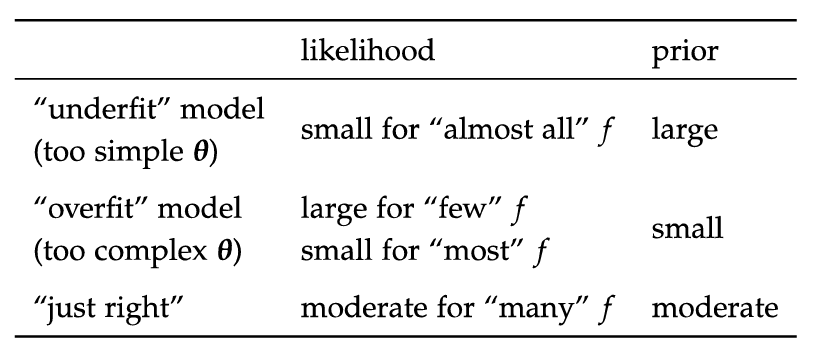
\includegraphics[width=\linewidth]{chapter_figs/04_figs/table.png}
    \column{0.4\textwidth}
    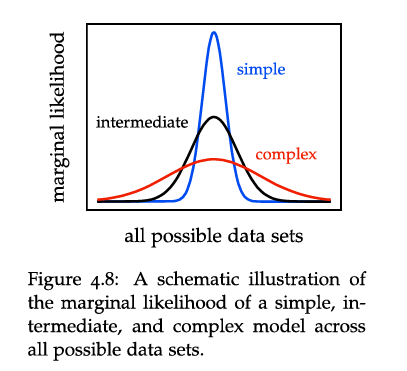
\includegraphics[width=0.8\linewidth]{chapter_figs/04_figs/f48.png}
\end{columns}




\pause
\vspace{0.3cm}
\textbf{Conclusion:} Maximizing marginal likelihood automatically balances these two forces. 
\end{frame}

\begin{frame}{Marginal Likelihood for GPs}
\vspace{-0.2cm}
\textbf{Recall from GP prior:}
\[
y_{1:n} \mid x_{1:n}, \theta \sim \mathcal{N}(0, K_{f,\theta} + \sigma_n^2 I) \tag{4.27}
\]

Let $K_{y,\theta} = K_{f,\theta} + \sigma_n^2 I$

\pause
\vspace{0.3cm}
Then the marginal likelihood becomes:
\[
p(y \mid x, \theta) = \mathcal{N}(y \mid 0, K_{y,\theta})
\]

Taking negative log:
\[
\mathcal{L}(\theta) = \frac{1}{2} y^\top K_{y,\theta}^{-1} y + \frac{1}{2} \log \det K_{y,\theta} + \frac{n}{2} \log 2\pi \tag{4.28}
\]

\pause
\textbf{Breaking this down:}
\begin{itemize}
    \item $\boxed{y^\top K^{-1} y}$ — data fit (how well predictions match $y$)
    \item $\boxed{\log \det K}$ — model complexity penalty
    \item Constant term $\frac{n}{2} \log 2\pi$ — does not depend on $\theta$
\end{itemize}
\end{frame}

\begin{frame}{Marginal Likelihood for GPs}

Drop the constant \rightarrow \, final objective:
\[
\hat{\theta}_{\text{MLE}} = \arg\min_\theta \left(
\frac{1}{2} y^\top K_{y,\theta}^{-1} y + \frac{1}{2} \log \det K_{y,\theta}
\right) \tag{4.29}
\]
\end{frame}

\begin{frame}{Gradient of Log Marginal Likelihood}
To optimize $\mathcal{L}(\theta)$, we need the gradient $\frac{\partial}{\partial \theta_j} \log p(y \mid x, \theta)$.

\vspace{0.3cm}
\textbf{GPs allow this in closed form:}
\[
\frac{\partial}{\partial \theta_j} \log p(y \mid x, \theta)
= \frac{1}{2} \text{tr}\left[
\left( \boldsymbol{\alpha} \boldsymbol{\alpha}^\top - K^{-1}_{y,\theta} \right)
\frac{\partial K_{y,\theta}}{\partial \theta_j}
\right] \tag{4.30}
\]

\pause
\textbf{Where:}
\begin{itemize}
    \item $\boldsymbol{\alpha} = K_{y,\theta}^{-1} y$
    \item $\frac{\partial K_{y,\theta}}{\partial \theta_j}$ is the derivative of the kernel matrix w.r.t. hyperparameter $\theta_j$
    \item $\text{tr}(M)$ = trace of matrix $M$ (sum of diagonal elements)
\end{itemize}

\vspace{0.3cm}
This allows gradient-based optimization (e.g. Adam, SGD).
\end{frame}

\begin{frame}{MAP and Full Bayesian Treatment of $\theta$}
\textbf{MLE:} finds the best $\theta$ by maximizing $p(y \mid x, \theta)$, when no prior knowledge about $\theta$

\pause
\textbf{MAP:} adds a prior over $\theta$:
\[
\hat{\theta}_{\text{MAP}} = \arg\max_\theta \, p(\theta) \cdot p(y \mid x, \theta) \tag{4.31}
\]

Taking log:
\[
= \arg\min_\theta \left(
- \log p(\theta) - \log p(y \mid x, \theta)
\right) \tag{4.32}
\]

\pause
\textbf{Fully Bayesian:} integrate out $\theta$
\[
p(y^* \mid x^*, \mathcal{D}) =
\int \int p(y^* \mid x^*, f) \cdot p(f \mid \mathcal{D}, \theta) \cdot p(\theta) \, df \, d\theta \tag{4.33}
\]

\textbf{Challenge:} This integral is intractable in most practical cases.

\pause
So we often settle for MLE or MAP, or use variational approximations.
\end{frame}

\begin{frame}{4.5 Why Do We Need Approximations?}
\textbf{Key issue: Computational Cost}

\begin{itemize}
    \item Gaussian Processes require inversion of an $n \times n$ matrix.
    \item This costs:
    \[
    \mathcal{O}(n^3)
    \]
    \item For large datasets ($n \sim 10^4$ or more), this becomes very slow.
    \item In contrast, Bayesian linear regression has lower cost:
    \[
    \mathcal{O}(nd^2)
    \quad \text{where } d = \text{input feature dimension}
    \]
    \item Therefore, we look for ways to \textbf{approximate} a GP while preserving performance.
\end{itemize}

\vspace{0.3cm}
\textcolor{gray}{Next: What happens when optimization isn't even guaranteed to find a global solution?}
\end{frame}


\begin{frame}{MLL Surface and Two GP Fits}
\begin{columns}
\column{0.55\textwidth}
\textbf{Top plot:} Contour plot of negative log marginal likelihood (MLL)

\begin{itemize}
    \item Axes: Lengthscale $h$ vs noise std $\sigma_n$
    \item Two '+' marks: local optima found during optimization
    \item Shows that MLL can have multiple optima
\end{itemize}

\pause
\vspace{0.3cm}
\textbf{Bottom plots:} GP regression fits corresponding to the two optima

\begin{itemize}
    \item Left: small lengthscale, flexible model \rightarrow \, smooth interpolation
    \item Right: large noise, rigid model \rightarrow \, explains variation as noise
\end{itemize}

\column{0.4\textwidth}
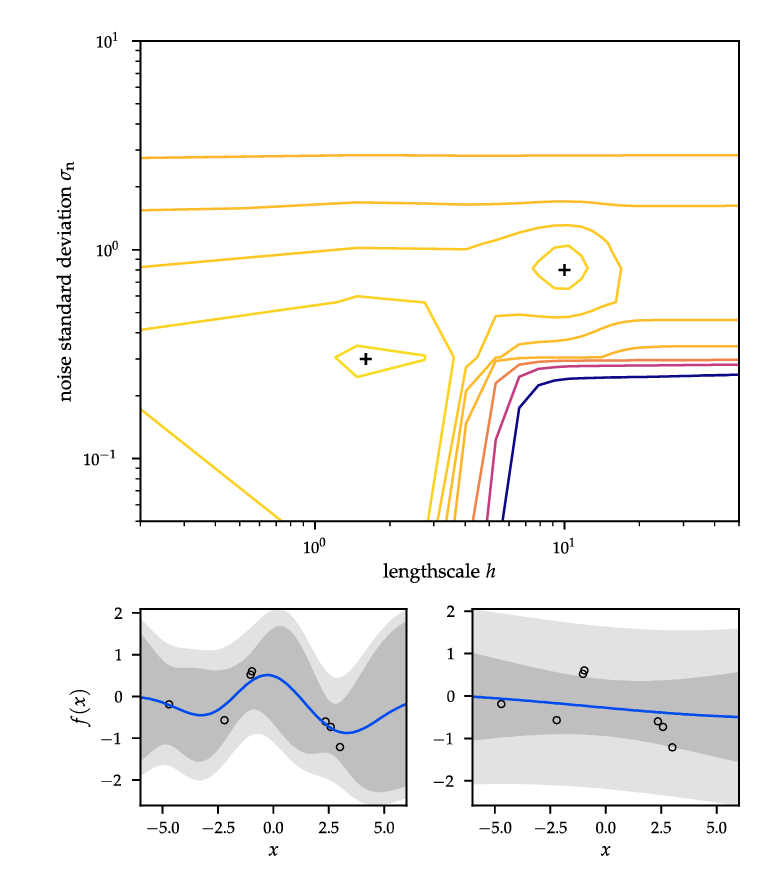
\includegraphics[width=0.8\linewidth]{chapter_figs/04_figs/f410.png}
\end{columns}

\vspace{0.3cm}
\textbf{Takeaway:} Hyperparameter learning is sensitive to initialization and optimization.
\end{frame}

\begin{frame}{4.5.1 Local Methods}
\begin{itemize}
    \item Forward sampling from a GP requires conditioning on all previous observations.
    \item This becomes computationally expensive as $n$ grows.
    \item One idea: Only condition on points “near” the test input $x$.
    \item For example: keep only points $x'$ such that
    \[
    |k(x, x')| \geq \tau \quad \text{for some threshold } \tau > 0
    \]
    \item This “cuts off the tails” of the kernel — treating distant points as independent.
\end{itemize}

\pause
\vspace{0.2cm}
\textbf{Benefit:} Reduces computation.

\textbf{Caution:} If $\tau$ is too large, we may lose important long-range correlations.

\vspace{0.2cm}
This is an example of a \textbf{sparse approximation} to a GP.
\end{frame}

\begin{frame}{4.5.2 Kernel Function Approximation}
\textbf{Goal:} Approximate the kernel $k(x, x')$ directly using a low-dimensional feature map.

\vspace{0.2cm}
\textbf{Idea:}
\[
k(x, x') \approx \phi(x)^\top \phi(x') \tag{4.34}
\]

Then, apply Bayesian linear regression on $\phi(x)$ instead of GPs.

\vspace{0.3cm}
\textbf{Computational benefit:} Time complexity becomes:
\[
\mathcal{O}(nm^2 + m^3)
\]
where $m$ is the number of features.

\vspace{0.3cm}
\pause
This leads us to \textbf{Random Fourier Features (RFF)}, where:
- The feature map $\phi(x)$ is constructed from sine and cosine of random projections
- Based on Fourier transform theory and Bochner's theorem
\end{frame}

\begin{frame}{Fourier View of Kernels}
\textbf{Euler's identity:}
\[
e^{ix} = \cos x + i \sin x \tag{4.35}
\]

\textbf{Fourier transform:}
\[
\hat{f}(\xi) = \int_{\mathbb{R}^d} f(x) e^{-2\pi i \xi^\top x} \, dx \tag{4.36}
\]
\[
f(x) = \int_{\mathbb{R}^d} \hat{f}(\xi) e^{2\pi i \xi^\top x} \, d\xi \tag{4.37}
\]

\pause
\textbf{Stationary kernel as function of } $x - x'$:
\[
k(x - x') = \int_{\mathbb{R}^d} p(\omega) e^{i \omega^\top (x - x')} d\omega \tag{4.38}
\]
Bochner's theorem: $p(\omega)$ is the spectral density of $k$.

\pause
\textbf{Gaussian kernel’s spectral density:}
\[
p(\omega) = (2h^2 \pi)^{d/2} \exp \left( - h^2 \|\omega\|^2 / 2 \right) \tag{4.39}
\]
\end{frame}


\begin{frame}{Random Fourier Features Approximation}
Use Monte Carlo sampling over $\omega \sim p(\omega)$ and $b \sim \text{Unif}[0, 2\pi]$.

\textbf{Define:}
\[
z_{\omega, b}(x) = \sqrt{2} \cos(\omega^\top x + b)
\]

Then:
\[
k(x, x') \approx z(x)^\top z(x') \tag{4.42}
\]
\[
z(x) = \frac{1}{\sqrt{m}} \begin{bmatrix}
z_{\omega^{(1)}, b^{(1)}}(x) \\
\vdots \\
z_{\omega^{(m)}, b^{(m)}}(x)
\end{bmatrix} \tag{4.43}
\]

\vspace{0.3cm}
\textbf{Theorem 4.13:} This approximation converges uniformly to the true kernel as $m \to \infty$

\textbf{Benefit:} Fast kernel approximation, scalable GPs!
\end{frame}

\begin{frame}{4.5.3 Inducing Point Methods: Motivation}
\textbf{Problem:} Using all $n$ training points in a GP is expensive.

\vspace{0.2cm}
\textbf{Idea:} Use a smaller set of \textbf{inducing points} to summarize the full data.

\[
U \triangleq \{\bar{x}_1, \dots, \bar{x}_k\}
\quad \text{where } k \ll n
\]

\vspace{0.3cm}
\textbf{We model:}
\[
u \triangleq \begin{bmatrix} f(\bar{x}_1) & \cdots & f(\bar{x}_k) \end{bmatrix}^\top
\quad \sim \mathcal{N}(0, K_{UU})
\]

\vspace{0.3cm}
\textbf{Recover full GP using marginalization:}
\[
p(f^*, f) = \int p(f^*, f \mid u) \, p(u) \, du \tag{4.45}
\]

\pause
This lets us reduce computations while preserving most information.
\end{frame}

\begin{frame}{Subset of Regressors}
\textbf{Approximation:} Assume $f$ and $f^*$ are conditionally independent given $u$:
\[
p(f^*, f) \approx \int p(f^* \mid u) \, p(f \mid u) \, p(u) \, du \tag{4.46}
\]

\pause
\textbf{From Gaussian conditionals:}
\begin{align*}
p(f \mid u) &\sim \mathcal{N}(K_{AU} K_{UU}^{-1} u, \, K_{AA} - Q_{AA}) \tag{4.47a} \\
p(f^* \mid u) &\sim \mathcal{N}(K_{\ast U} K_{UU}^{-1} u, \, K_{\ast\ast} - Q_{\ast\ast}) \tag{4.47b}
\end{align*}

Where $Q_{ab} = K_{aU} K_{UU}^{-1} K_{Ub}$

\pause
\textbf{Subset of Regressors (SoR):} keep the mean and drop the variances/covariances
\begin{align*}
q_{\text{SoR}}(f \mid u) &= \mathcal{N}(K_{AU}K_{UU}^{-1}u, 0) \tag{4.48a} \\
q_{\text{SoR}}(f^* \mid u) &= \mathcal{N}(K_{\ast U}K_{UU}^{-1}u, 0) \tag{4.48b}
\end{align*}
\textbf{Drawback}: Since we drop the uncertainties in this approach, therefore, we may unrealistic predictions.
\end{frame}

\begin{frame}{Fully Independent Training Conditional}
\pause
\textbf{FITC (Fully Independent Training Conditional):}
\begin{align*}
q_{\text{FITC}}(f \mid u) &= \mathcal{N}(K_{AU}K_{UU}^{-1}u, \, \text{diag}(K_{AA} - Q_{AA})) \tag{4.49a} \\
q_{\text{FITC}}(f^* \mid u) &= \mathcal{N}(K_{\ast U}K_{UU}^{-1}u, \, \text{diag}(K_{\ast\ast} - Q_{\ast\ast})) \tag{4.49b}
\end{align*}

\pause
\textbf{Summary:}
\begin{itemize}
    \item SoR: keeps mean, discards all variance
    \item FITC: keeps mean + variances, ignores off-diagonal covariances
\end{itemize}
\end{frame}

\begin{frame}{Graph: SoR vs FITC}
\begin{figure}
    \centering
    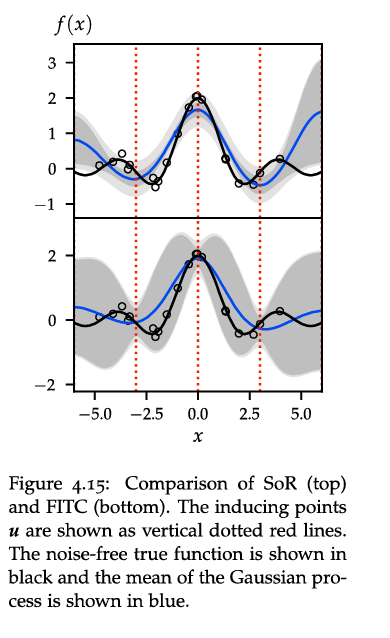
\includegraphics[width=0.3\linewidth]{chapter_figs/04_figs/sor_fitc.png}
\end{figure}

    
\end{frame}

\begin{frame}{Discussion: GP Approximations in Practice}
\begin{itemize}
    \item GPs are flexible non-parametric models that reason over functions.
    \item But exact inference becomes costly with large datasets.
\end{itemize}

\vspace{0.3cm}
\textbf{This chapter introduced several ways to approximate GPs:}
\begin{itemize}
    \item \textbf{Local methods:} Use only nearby data points
    \item \textbf{Kernel approximations:} RFF via Bochner’s theorem
    \item \textbf{Inducing points:} Summarize data through select locations
\end{itemize}

\vspace{0.2cm}
\textbf{Next:} We explore how to combine these probabilistic ideas with scalable models.
\end{frame}














{\usebackgroundtemplate{
\includegraphics[width=\paperwidth]{chapter_figs/03_figs/thankyou.png}}
	\begin{frame}[plain,noframenumbering]
	\end{frame}}



\end{document}